\begingroup
\setlength{\tabcolsep}{0pt}
\renewcommand{\arraystretch}{1} % Default value: 1
\setlength{\fboxsep}{1.8mm}
\begin{table*}
\centering
\begin{tabular}{|P{2cm}|P{1.5cm}|P{2cm}|P{1.5cm} B P{1.5cm}|P{7cm}|}
\hline
Technique & Interval & Reduction & Data  &  Avg$_{L2}$ & Cell & Scatter Plot \\
& & & (MB) & & Side\% & \multirow{6}{*}{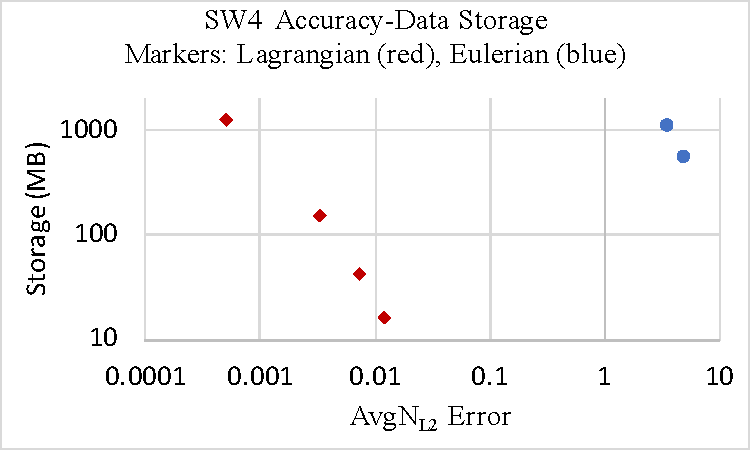
\includegraphics[width=0.95\linewidth]{images/sw4_accuracy.pdf}} \\
\cline{1-6}
\multirow{2}{*}{\textcolor{blue!85}{\textbf{Eulerian}}} & 250 & \multirow{2}{*}{Full Res} & 1100 & 3.5714 & 0.922 & \\
\cline{2-2}\cline{4-6}
 & 500 & & 550  & 5.0493 & 1.302  & \\
\cline{1-6}
\multirow{4}{*}{\textcolor{BrickRed}{\textbf{Lagrangian}}} & \multirow{4}{*}{250} & 1:1 & 1300 & 0.0005 & 0.0001  &  \\ 
\cline{3-6}
 &  & 1:8 & 158 & 0.0033 & 0.0008 &  \\
\cline{3-6}
 &  & 1:27 & 42 & 0.0072 & 0.0018 & \\
\cline{3-6}
 &  & 1:64 & 16 & 0.0128 & 0.0031 &  \\
\hline
\end{tabular}
\caption{SW4 Accuracy Results. Simulation grid dimensions are $1001\times1001\times276$. We run these experiments for 2000 cycles. We calculate the reconstruction accuracy of 90,000 massless test particles that we place in between $Z=5000$ and $Z=15000$. }
\end{table*}
\endgroup
